\documentclass[11pt,a4paper]{article}
\usepackage[utf8]{inputenc}
\title{Preparatório 7 - Eletrônica}
\author{Hiago Riba Guedes RGU:11620104}
\date{Professor:Guilherme Garcia}
\usepackage{graphicx}
\usepackage{subfigure}
\graphicspath{{/home/hiago/Videos/Prep7/}}

\begin{document}
\maketitle

Diodos usados :BY 127 -diodo retificador\\
BZX 79 C5 V6 - diodo zener\\\\
Dados pertinentes:\\
BY 127:\\
$V_{rms_{max}}$=875 V\\
Máxima correte direta=1A\\\\
Fonte:http://www.circuitstoday.com/wp-content/uploads/2009/03/by127.pdf\\
\\
BZX79C5V6:\\
$V_{zener}$=min=5.2 V ; max=6 V\\
$I_{zener}$=5 mA\\
$Z_{max}$=40$\Omega$\\

Fonte:http://www.circuitstoday.com/wp-content/uploads/2009/03/by127.pdf\\
\\Como o LT Spice não tem esses componentes será utilizado componenentes similares , o resultado gráfico será o mesmo mas os valores das coordenadas deverá ser diferente.\\

\begin{figure}[!htb]

\includegraphics[scale=0.5]{1}
1-Ceifador positivo \\
\end{figure} 
\begin{figure}[!htb]

\includegraphics[scale=0.5]{2}
2-Ceifador positivo e negativo \\
\end{figure} 
\begin{figure}[!htb]

\includegraphics[scale=0.5]{3}
3-Grafico positivo e negativo \\
\end{figure} 
\begin{figure}[!htb]

\includegraphics[scale=0.5]{4}
4-ceifador deslocado pra cima \\
\end{figure} 
\begin{figure}[!htb]

\includegraphics[scale=0.5]{5}
5-Inverso da 4 \\
\end{figure} 
\begin{figure}[!htb]

\includegraphics[scale=0.5]{6}
6-Meia onda e ceifador com zener \\
\\Com o diodo especificado o $V_z$ é de 5,6 V.Então os limites de ceifamento estariam na faixa de 5.6 V,nesse caso para cima.
\end{figure} 
\begin{figure}[!htb]
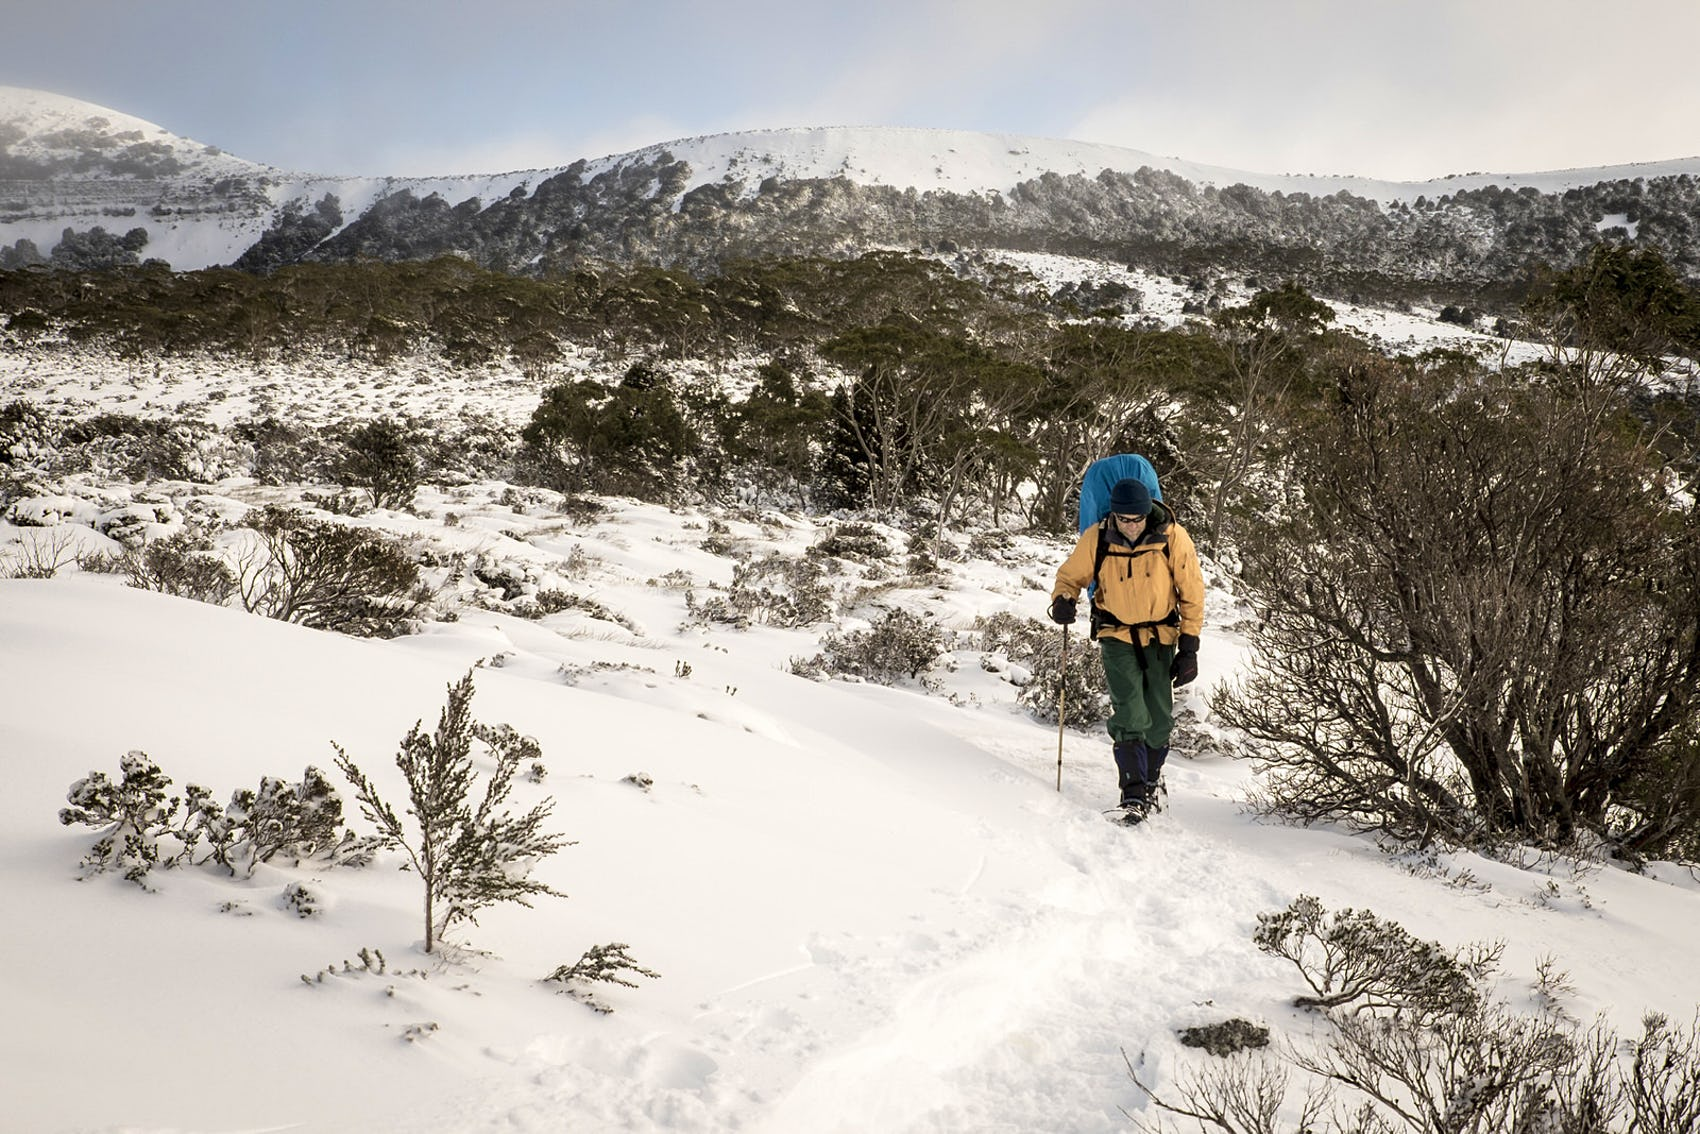
\includegraphics[scale=0.5]{7}
7-Ceifador positivo e negativo com zener \\
\\Com o diodo especificado o $V_z$ é de 5,6 V.Então os limites de ceifamento estariam na faixa de 5.6 V,nesse caso para baixo e para cima.
\end{figure} 

\end{document}